\section{Word Frequency}
\label{appendix2}

The following charts show how often some of the words related to `third sex/gender' and to `sex/gender-characteristics' are used in the Pali Canon and commentaries as well as in the Sanskrit, Chinese and Tibetan texts. In the Figures, the (b) charts show the relative number of words. This takes into account the size of the specific parts of the Canon and Commentaries.\footnote{The total number of words in a collection is divided by the total number of characters in that collection times 10\textsuperscript{5} (Pali and Tibetan) and 10\textsuperscript{11} (Sanskrit). For the Chinese no charts are given for the relative number of words because there was no significant difference with the charts for the total number of words. For the Tibetan no charts are given for words relating to the characteristics of sex/gender due to a lack of data.}

\captionsetup{justification   = raggedright,
              singlelinecheck = false}

\subsection{Words denoting gender-nonconforming individuals}
\label{appendix2a}
\subsubsection*{Pali Canon and Commentaries}

The Pali charts use the data from the \href{https://buddhanexus.net}{BuddhaNexus.net} database, which comprises the data from \href{https://suttacentral.net/}{SuttaCentral.net} and \href{https://tipitaka.org/}{VRI--Vipassana Research Institute}.

\begin{figure}[!h]
  \begin{subfigure}{0.564\linewidth}
    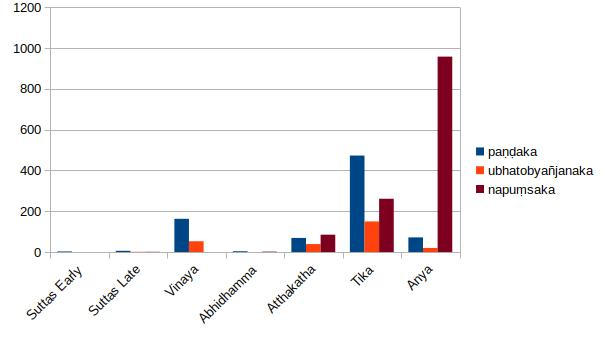
\includegraphics[width=\linewidth]{pali.jpg}
    \caption{Total number of words.}
  \end{subfigure}
  \hfill
  \begin{subfigure}{0.436\linewidth}
    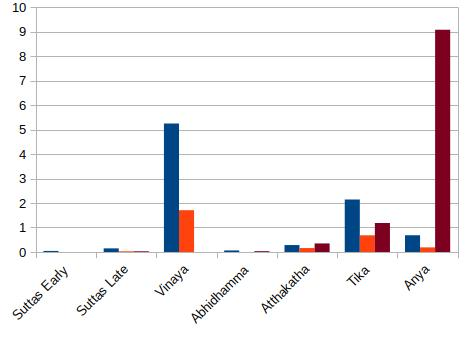
\includegraphics[width=\linewidth]{pali_weighted.jpg}
    \caption{Relative number of words.}
  \end{subfigure}
\setcounter{figure}{2}
\captionof{figure}{Words denoting gender-nonconforming individuals in the Pali Canon and Commentaries.}
\label{pali1}
\end{figure}

\begin{figure}[!h]
  \begin{subfigure}{\linewidth}
  \begin{center}
    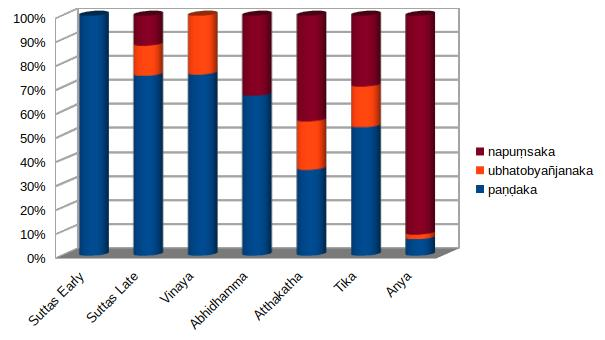
\includegraphics[width=0.5\linewidth]{pali_perc.jpg}
  \end{center}
  \end{subfigure}
\setcounter{figure}{3}
\captionof{figure}{Relative importance of words within each collection (as a percentage).}
\label{pali2}
\end{figure}

\newpage
\subsubsection*{Sanskrit Buddhist and Vedic Canon and Commentaries}

The Sanskrit charts use the data from the \href{https://buddhanexus.net}{BuddhaNexus.net} database, which comprises the data from \href{http://gretil.sub.uni-goettingen.de/gretil.html}{GRETIL--Göttingen Register of Electronic Texts in Indian Languages}. The data from the \href{http://www.dsbcproject.org/}{DSBC--Digital Sanskrit Buddhist Canon} is not included in these charts because they largely overlap with the GRETIL data which would result in double entries.

Unlike the texts in the Pali, Chinese and Tibetan canons, the GRETIL data used for the Sanskrit charts does not comprise the entire Buddhist Canon. They are also not ordered by approximate lateness. The Vedic/Brahmanical texts are also included in these charts.\footnote{Note that the prominance of the relative number of words in the category `Buddhist Misc.' is mainly due to the very small size of this category.}

\begin{figure}[!h]
  \begin{subfigure}{0.558\linewidth}
    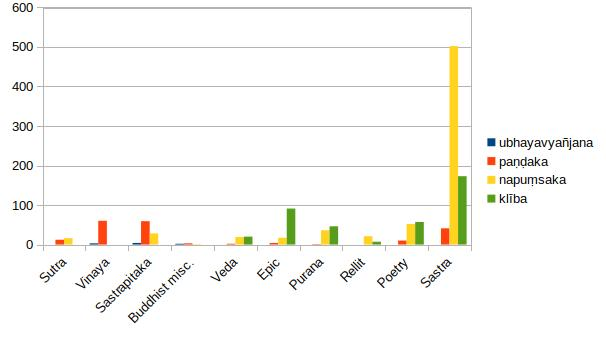
\includegraphics[width=\linewidth]{sanskrit.jpg}
    \caption{Total number of words.}
  \end{subfigure}
  \hfill
  \begin{subfigure}{0.442\linewidth}
    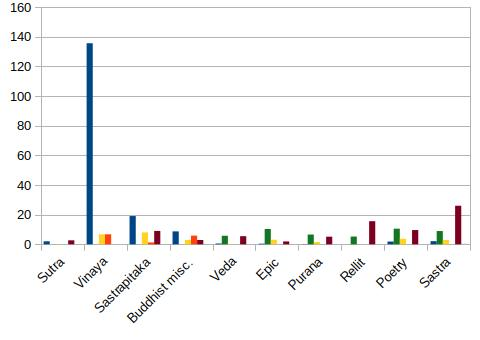
\includegraphics[width=\linewidth]{sanskrit_weighted.jpg}
    \caption{Relative number of words.}
  \end{subfigure}
\setcounter{figure}{4}
\captionof{figure}{Words denoting gender-nonconforming individuals in the Sanskrit Buddhist and Vedic Canon and Commentaries.}
\label{sanskrit1}
\end{figure}

\begin{figure}[!h]
  \begin{subfigure}{\linewidth}
  \begin{center}
    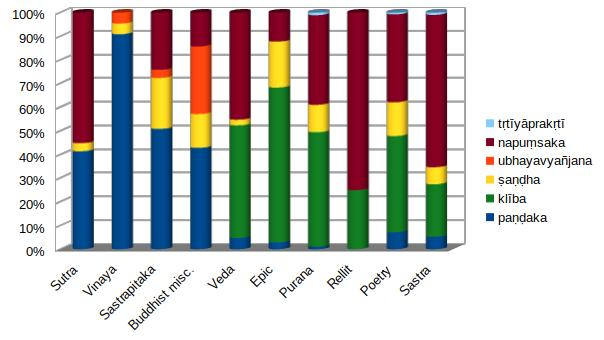
\includegraphics[width=0.5\linewidth]{sanskrit_perc.jpg}
  \end{center}
  \end{subfigure}
\setcounter{figure}{5}
\captionof{figure}{Relative importance of words within each collection (as a percentage).}
\label{sanskrit2}
\end{figure}

\newpage
\subsubsection*{Chinese Buddhist Taishō Canon}

The Chinese charts use the data from the \href{https://buddhanexus.net}{BuddhaNexus.net} database, which comprises the data from \href{https://www.cbeta.org/}{CBETA--Chinese Buddhist Electronic Text Association}.

\begin{figure}[!h]
  \begin{subfigure}{\linewidth}
    \begin{center}
    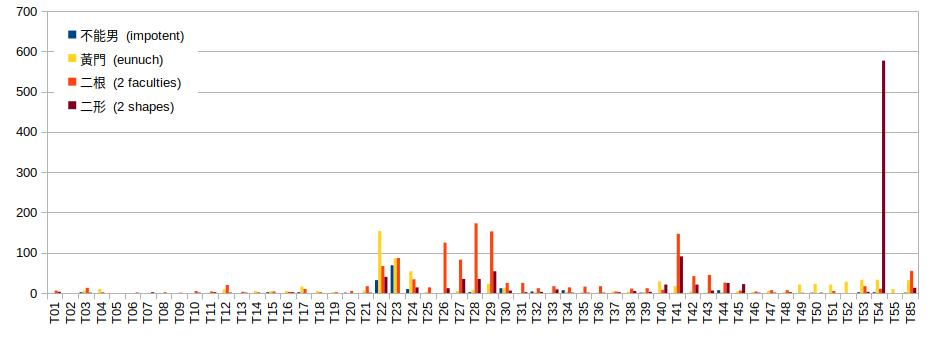
\includegraphics[width=0.9\linewidth]{chinese.jpg}
    \end{center}
  \end{subfigure}
\setcounter{figure}{6}
\captionof{figure}{Total number of words denoting gender-nonconforming individuals in the Chinese Taishō Canon.}
\label{chinese1}
\end{figure}

\begin{figure}[!h]
  \begin{subfigure}{\linewidth}
  \begin{center}
    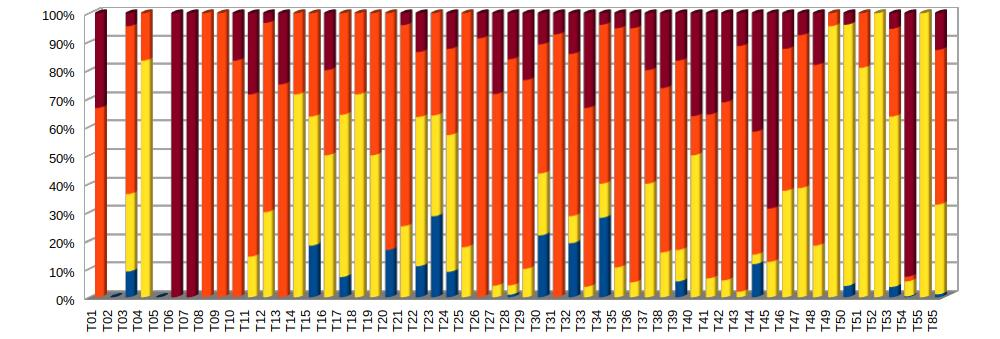
\includegraphics[width=0.98\linewidth]{chinese_perc.jpg}
  \end{center}
  \end{subfigure}
\setcounter{figure}{7}
\captionof{figure}{Relative importance of words within each collection (as a percentage).}
\label{chinese2}
\end{figure}

\newpage
\subsubsection*{Tibetan Buddhist Kangyur and Tengyur Canon}

The Tibetan charts use the data from the \href{https://buddhanexus.net}{BuddhaNexus.net} database, which comprises the data from \href{https://asianclassics.org/}{ACIP--Asian Classics Input Projects} and \href{https://www.tbrc.org/}{BDRC--Buddhist Digital Resource Center}.

\begin{figure}[!h]
  \begin{subfigure}{0.5\linewidth}
    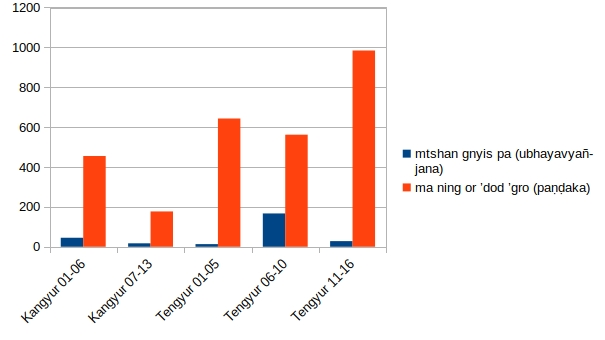
\includegraphics[width=\linewidth]{tibetan.jpg}
    \caption{Total number of words.}
  \end{subfigure}
  \hfill
  \begin{subfigure}{0.5\linewidth}
    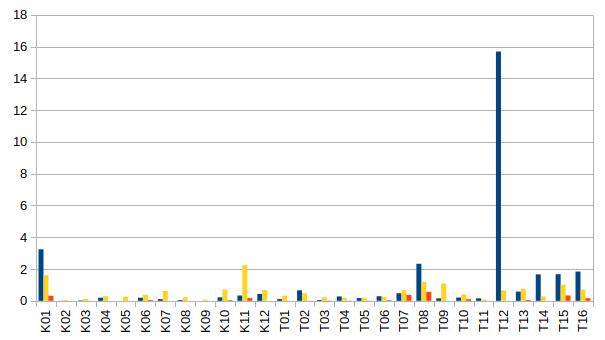
\includegraphics[width=\linewidth]{tibetan_weighted.jpg}
    \caption{Relative number of words.}
  \end{subfigure}
\setcounter{figure}{8}
\captionof{figure}{Words denoting gender-nonconforming individuals in the Tibetan Kangyur and Tengyur Canon.}
\label{tibetan1}
\end{figure}

\begin{figure}[!h]
  \begin{subfigure}{\linewidth}
  \begin{center}
    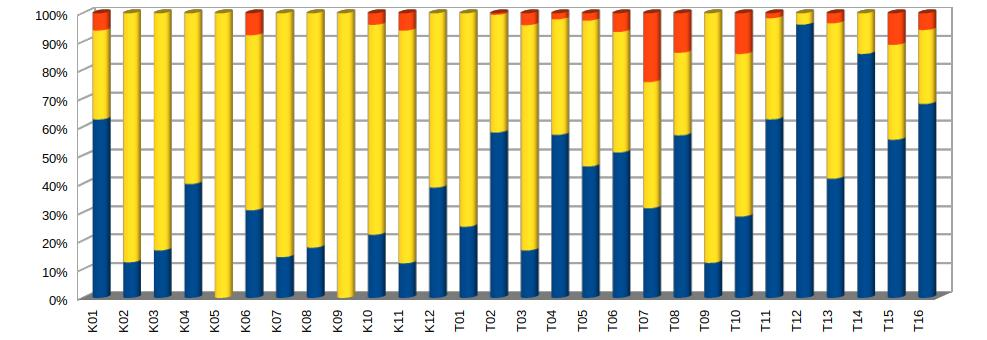
\includegraphics[width=0.9\linewidth]{tibetan_perc.jpg}
  \end{center}
  \end{subfigure}
\setcounter{figure}{9}
\captionof{figure}{Relative importance of words within each collection (as a percentage).}
\label{tibetan2}
\end{figure}

\newpage
\subsection{Words denoting sex/gender-characteristics}
\label{appendix2b}

In order to get an idea as to the frequency in which certain words are used to denote sex/gender characteristics as opposed to general characteristics I have used the prefixes \textit{itthi} (`female' Skt. \textit{strī}, Chn. 女) and \textit{purisa} (`male' Skt. \textit{puruṣa}, Chn. 男). 

\subsubsection*{Pali Canon and Commentaries}

\begin{figure}[!h]
  \begin{subfigure}{0.551\linewidth}
    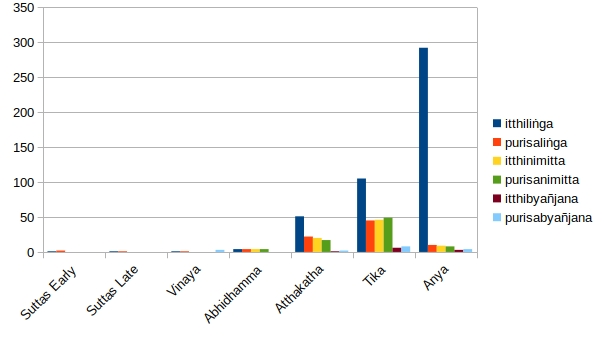
\includegraphics[width=\linewidth]{itthi.jpg}
    \caption{Total number of words.}
  \end{subfigure}
  \hfill
  \begin{subfigure}{0.449\linewidth}
    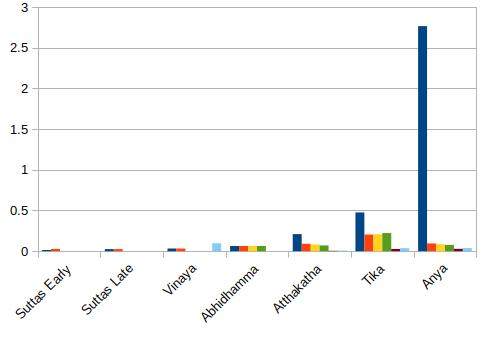
\includegraphics[width=\linewidth]{itthi_weighted.jpg}
    \caption{Relative number of words.}
  \end{subfigure}
\setcounter{figure}{10}
\captionof{figure}{Words denoting sex/gender-characteristics in the Pali Canon and Commentaries.}
\label{itthi}
\end{figure}

\begin{figure}[!h]
  \begin{subfigure}{\linewidth}
  \begin{center}
    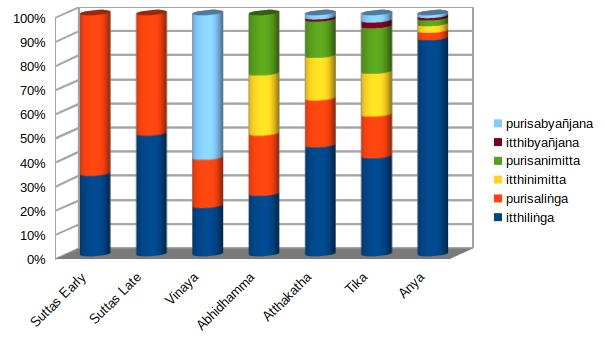
\includegraphics[width=0.38\linewidth]{itthi_perc.jpg}
  \end{center}
  \end{subfigure}
\setcounter{figure}{11}
\captionof{figure}{Relative importance of words within each collection (as a percentage).}
\label{itthi2}
\end{figure}

\begin{figure}[!h]
  \begin{subfigure}{0.496\linewidth}
    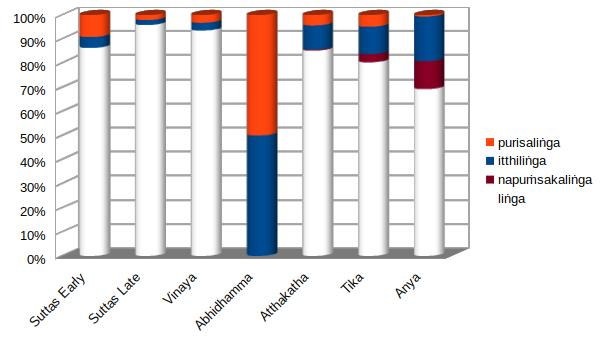
\includegraphics[width=\linewidth]{pali_linga.jpg}
    \caption{Liṅga in relation to words denoting sex/gender-characteristics.}
  \end{subfigure}
  \hfill
  \begin{subfigure}{0.504\linewidth}
    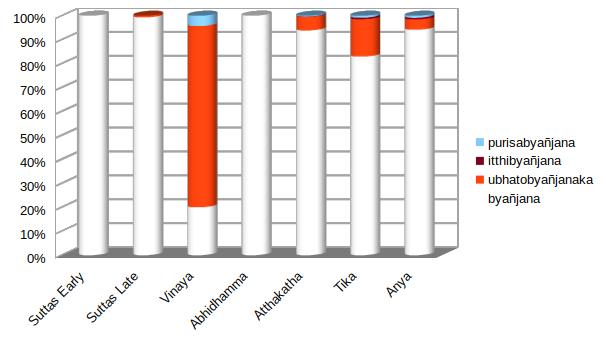
\includegraphics[width=\linewidth]{pali_byanyana.jpg}
    \caption{Byañjana in relation to words denoting sex/gender-characteristics.}
  \end{subfigure}
\setcounter{figure}{12}
\captionof{figure}{Relative importance with regards to the root words within each collection.}
\label{itthi3}
\end{figure}


\newpage
\subsubsection*{Sanskrit Buddhist and Vedic Canon and Commentaries}

\begin{figure}[!h]
  \begin{subfigure}{0.551\linewidth}
    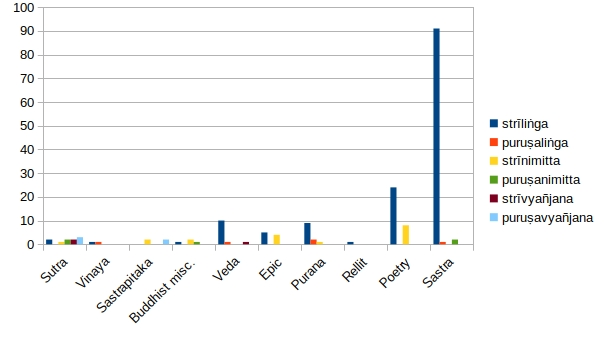
\includegraphics[width=\linewidth]{stri.jpg}
    \caption{Total number of words.}
  \end{subfigure}
  \hfill
  \begin{subfigure}{0.449\linewidth}
    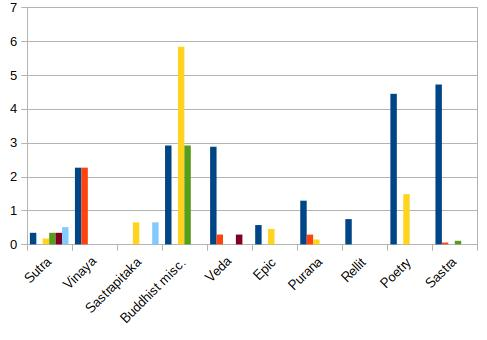
\includegraphics[width=\linewidth]{stri_weighted.jpg}
    \caption{Relative number of words.}
  \end{subfigure}
\setcounter{figure}{13}
\captionof{figure}{Words denoting sex/gender-characteristics in the Sanskrit Buddhist and Vedic Canons and Commentaries.}
\label{stri}
\end{figure}

\begin{figure}[!h]
  \begin{subfigure}{\linewidth}
  \begin{center}
    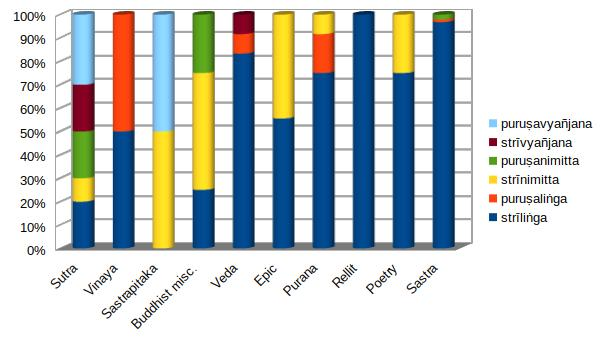
\includegraphics[width=0.5\linewidth]{stri_perc.jpg}
  \end{center}
  \end{subfigure}
\setcounter{figure}{14}
\captionof{figure}{Relative importance of words within each collection (as a percentage).}
\label{stri2}
\end{figure}

\begin{figure}[!h]
  \begin{subfigure}{0.497\linewidth}
    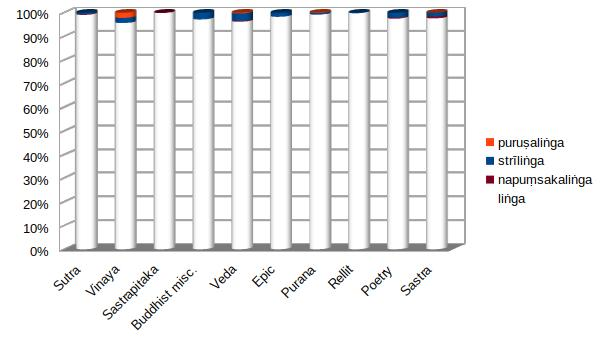
\includegraphics[width=\linewidth]{sanskrit_linga.jpg}
    \caption{Liṅga in relation to words denoting sex/gender-characteristics.}
  \end{subfigure}
  \hfill
  \begin{subfigure}{0.503\linewidth}
    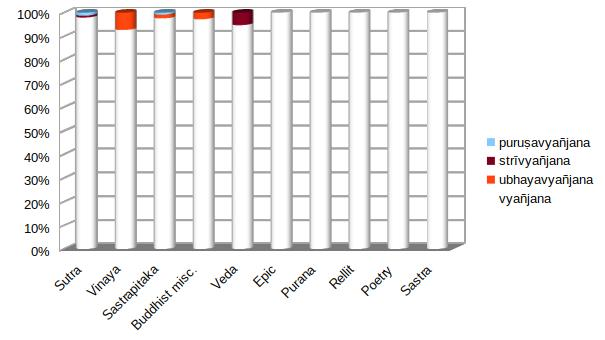
\includegraphics[width=\linewidth]{sanskrit_byanyana.jpg}
    \caption{Vyañjana in relation to words denoting sex/gender-characteristics.}
  \end{subfigure}
\setcounter{figure}{15}
\captionof{figure}{Relative importance with regards to the root words within each collection (as a percentage).}
\label{stri3}
\end{figure}


\newpage
\subsubsection*{Chinese Buddhist Taishō Canon}

\begin{figure}[!h]
  \begin{subfigure}{\linewidth}
    \begin{center}
    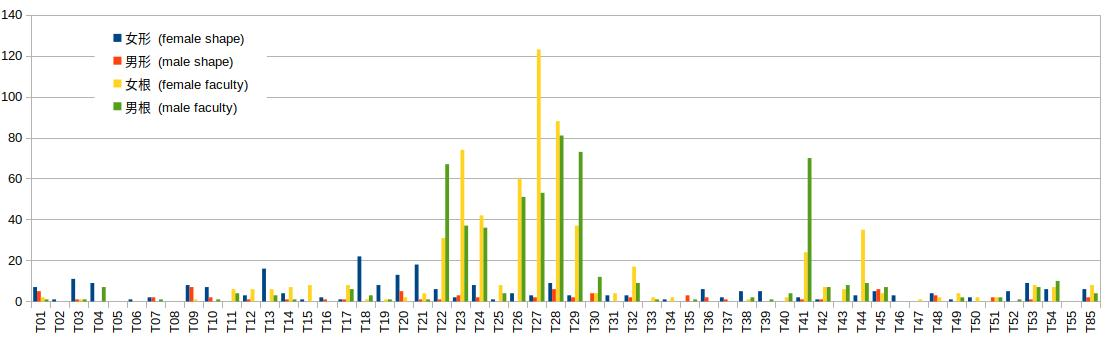
\includegraphics[width=0.73\linewidth]{chinese_itthi.jpg}
    \end{center}
  \end{subfigure}
\setcounter{figure}{16}
\captionof{figure}{Total number of words denoting sex/gender-characteristics in the Chinese Taishō Canon.}
\label{chinese3}
\end{figure}

\begin{figure}[!h]
  \begin{subfigure}{\linewidth}
  \begin{center}
    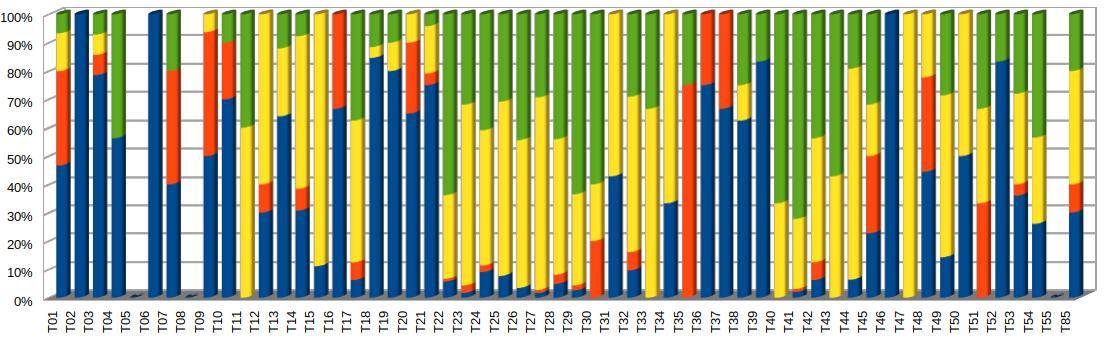
\includegraphics[width=0.75\linewidth]{chinese_itthi_perc.jpg}
  \end{center}
  \end{subfigure}
\setcounter{figure}{17}
\captionof{figure}{Relative importance of words within each collection (as a percentage).}
\label{chinese4}
\end{figure}

\begin{figure}[!h]
  \begin{subfigure}{\linewidth}
  \begin{center}
    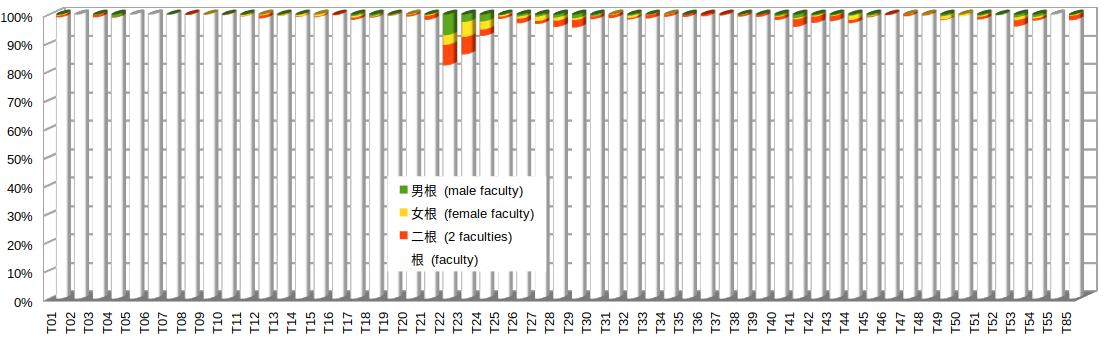
\includegraphics[width=0.75\linewidth]{chinese_faculty.jpg}
  \end{center}
  \end{subfigure}
\setcounter{figure}{18}
\captionof{figure}{Relative importance of words denoting sex/gender-characteristics with regards to the root word 根 (faculty) within each collection (as a percentage).}
\label{chinese5}
\end{figure}

\begin{figure}[!h]
  \begin{subfigure}{\linewidth}
  \begin{center}
    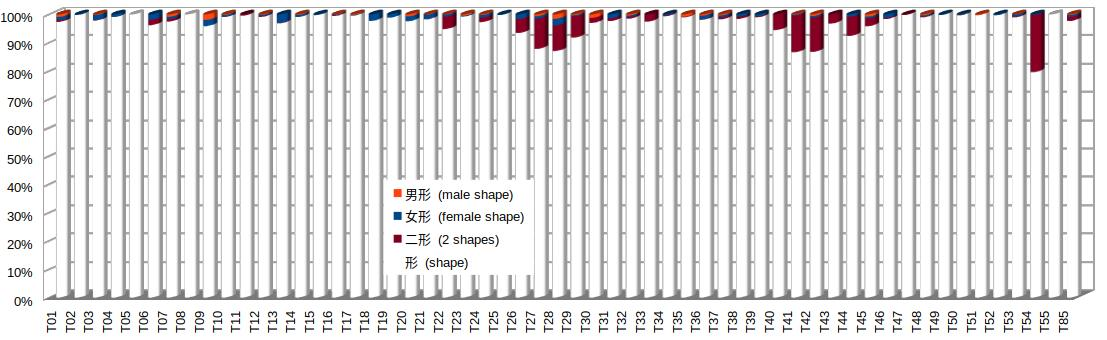
\includegraphics[width=0.75\linewidth]{chinese_shape.jpg}
  \end{center}
  \end{subfigure}
\setcounter{figure}{19}
\captionof{figure}{Relative importance of words denoting sex/gender-characteristics with regards to the root word 形 (shape) within each collection (as a percentage).}
\label{chinese6}
\end{figure}